% copyrights 2007 Dave Liu

%\documentclass[12pt]{beamer}
\documentclass[handout]{beamer}

\usepackage{amsmath}
\usepackage{amssymb} % http://www.ctan.org/tex-archive/macros/latex/required/psnfss/psnfss2e.pdf
\usepackage{helvet}
\usepackage{epsfig}

\usecolortheme{dolphin}
%\useoutertheme{infolines}



\title{A Benchmark Real Business Cycle Model} %  [A Benchmark Real Business Cycle Model
%\vskip 0.1in

%\subtitle{Dynamic Economic Theory (871)}
%\author[H Hollander]{Hylton Hollander}

%\institute[University of Stellenbosch]{\large{Department of Economics\\ University of Stellenbosch}}

\date{}
%\date[Feb. 25, 2014]{Mar. 05, 2014}

\begin{document}

\frame{\titlepage}

\frame{\frametitle{Contents:} \tableofcontents}




\begin{frame}

\frametitle{Readings} \vskip 0.1in

\begin{itemize}
\item Kydland, F. E. and E. C. Prescott, 1982. Time to build and
aggregate fluctuations. \emph{Econometrica}, 50 (6): 1345-1370.
\item Hansen, G. D., 1985. Indivisible labor and the business cycle.
\emph{Journal of Monetary Economics}, 16: 309-327.
\item Cooley, T. F. and E. C. Prescott, 1995. Economic growth and business
cycle. In Cooley, T. F., Frontier of business cycle research.
Princeton University Press. Princeton, New Jersey, pp 1-38.
\item A Toolkit for analyzing nonlinear dynamic stochastic models easily (by Uhlig
Harald).
\end{itemize}


\end{frame}

\section{Introduction: Economic Growth and Business Cycles}

\begin{frame}

\frametitle{Introduction: Economic Growth and Business Cycles}
\vskip 0.1in
%ref: Cooley (1995) CH1: 3-5
$\Box$ Kaldor's ``stylized facts" of growth (as characterized by
Solow (1970)): %%see Sims 2011 extra note in session 5 DET folder

\begin{enumerate}
\item Real output grows at a more or less constant rate;
\item The stock of real capital grows at a more or less constant
rate greater than the rate of growth of the labour input;
\item The growth rates of real output and the stock of capital tend
to be about the same;
\item The rate of profit on capital has a horizontal trend;
\item The rate of growth of output per-capita varies greatly from one
country to another;
\item Economies with a high share of profits in income tend to have a
high ratio of investment to output.
\end{enumerate}

\end{frame}

\begin{frame}

\frametitle{Introduction: Economic Growth and Business Cycles}
\vskip 0.1in

$\Box$ Kaldor's ``stylized facts" of growth (as characterized by
Solow (1970)):\\\vskip 0.1in

\textcolor{blue}{Remarks:}

\begin{itemize}
\item The 2nd and 3rd of these stylized facts imply that
investment-output ratio is constant;
\item The 3rd and 4th imply that
capital-output share is constant;
\item The first four together describe an economy experiencing``balanced
growth";
\item The 5th and 6th stylized facts have posed more difficulty for
neoclassical growth theory, and much of the modern endogenous growth
literature has been concerned with these features.
\end{itemize}


\end{frame}




\begin{frame}

\frametitle{Introduction: Economic Growth and Business Cycles}
\vskip 0.1in


$\Box$ Business cycle facts (Williamson, 2008)

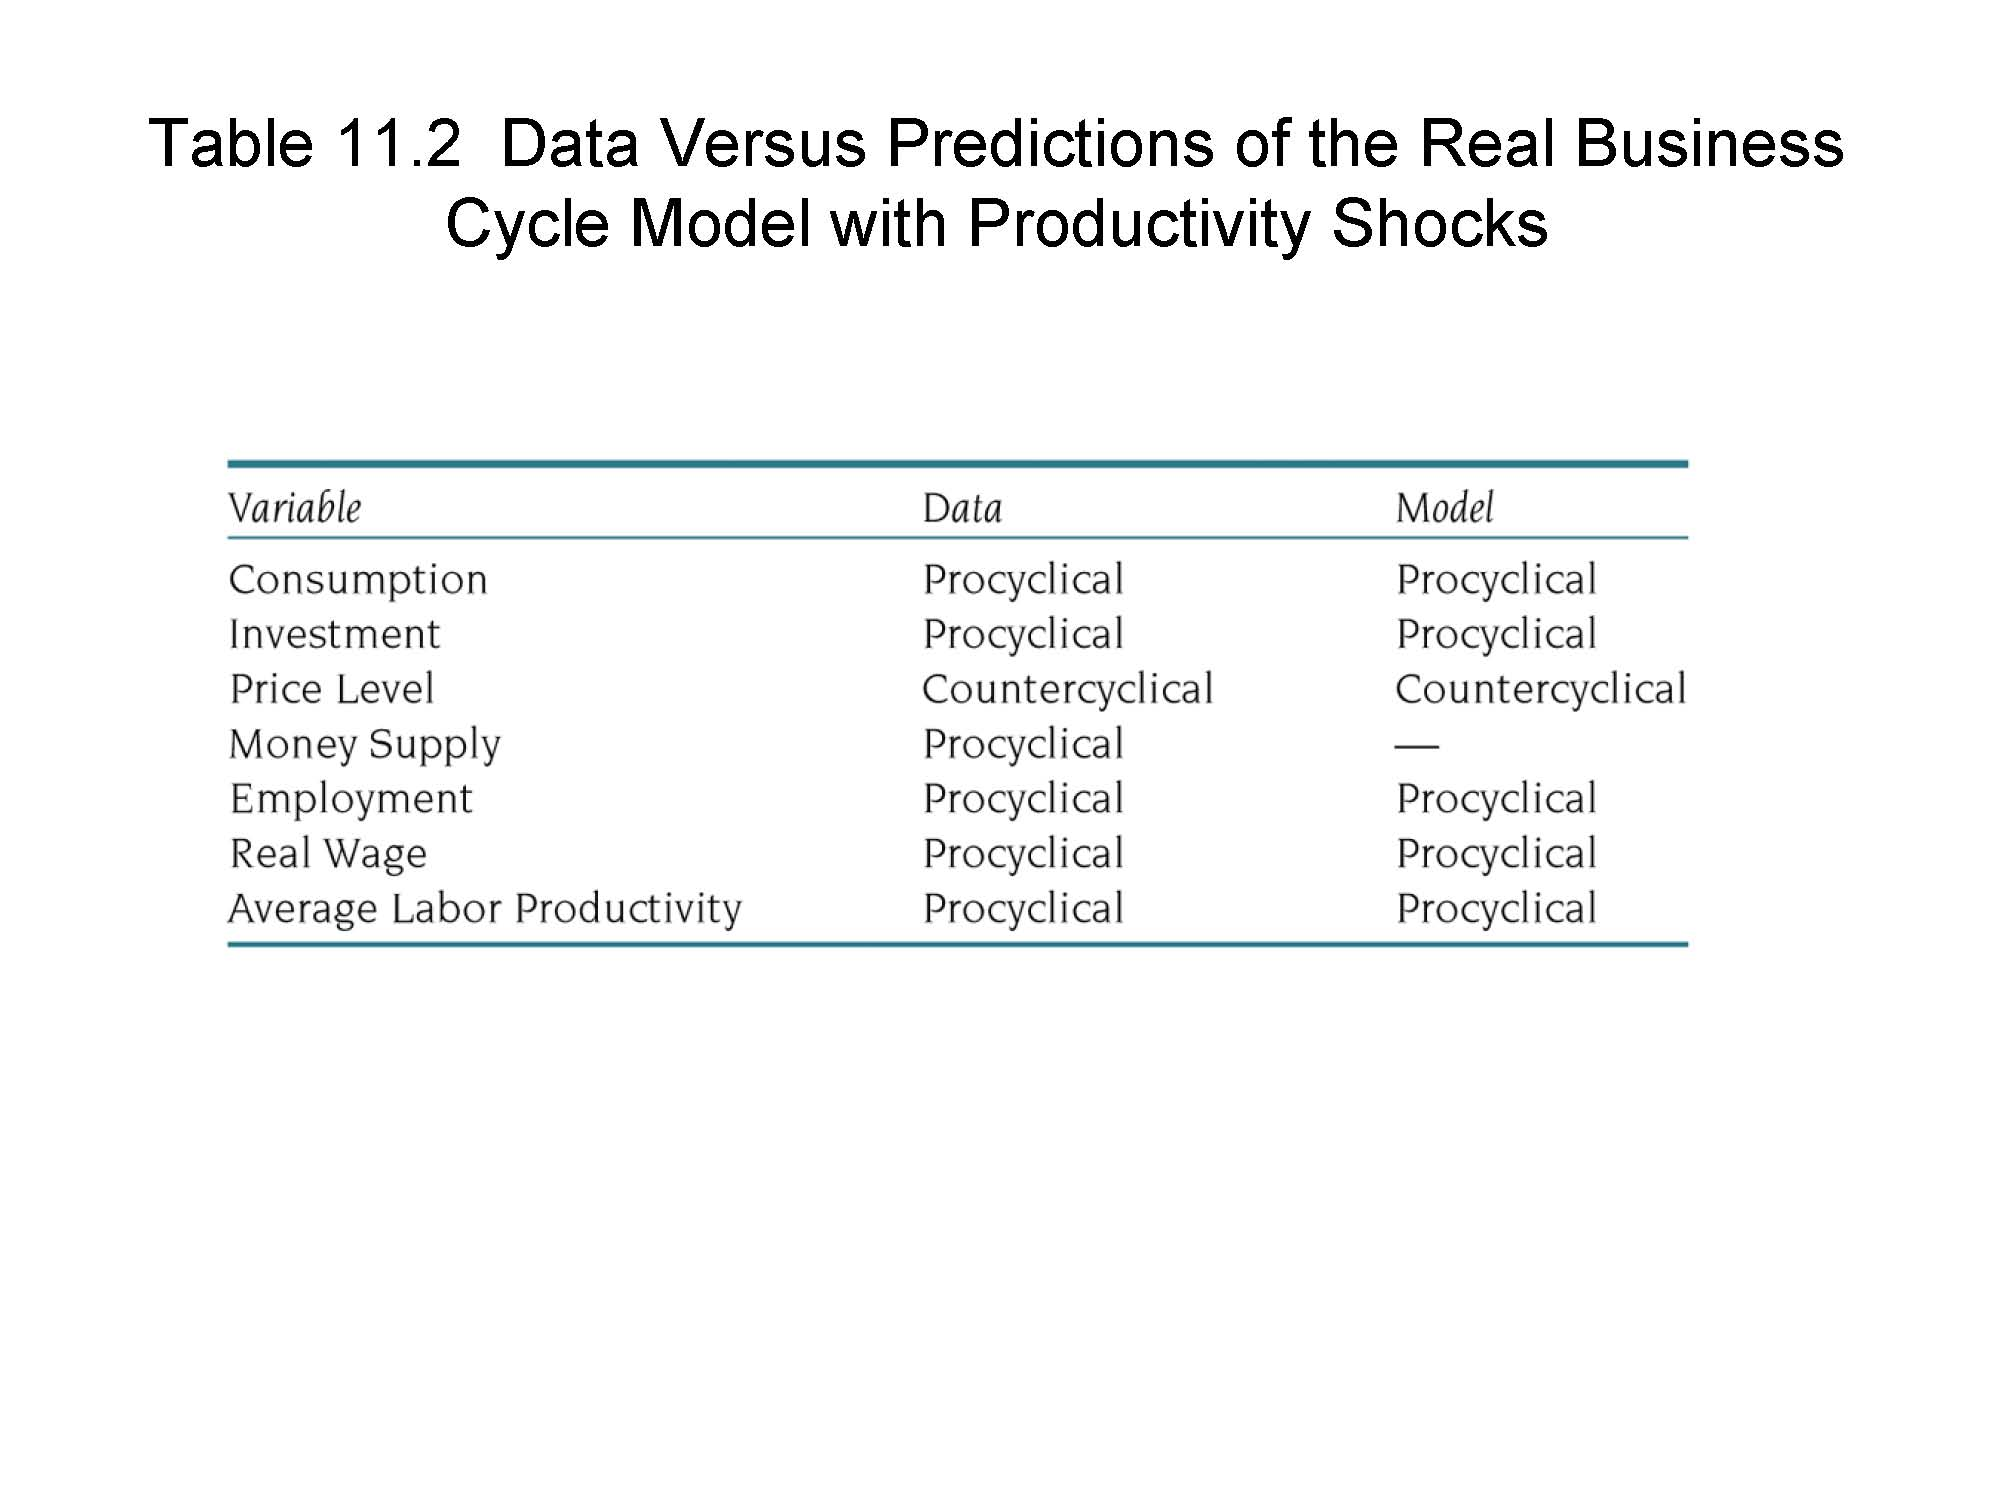
\includegraphics[width = 4.4in]{Tab11_2.jpg}


\end{frame}

\begin{frame}
{\scriptsize{$\Box$ Business cycle facts (Williamson, 2008)}}
\begin{figure}
\centering
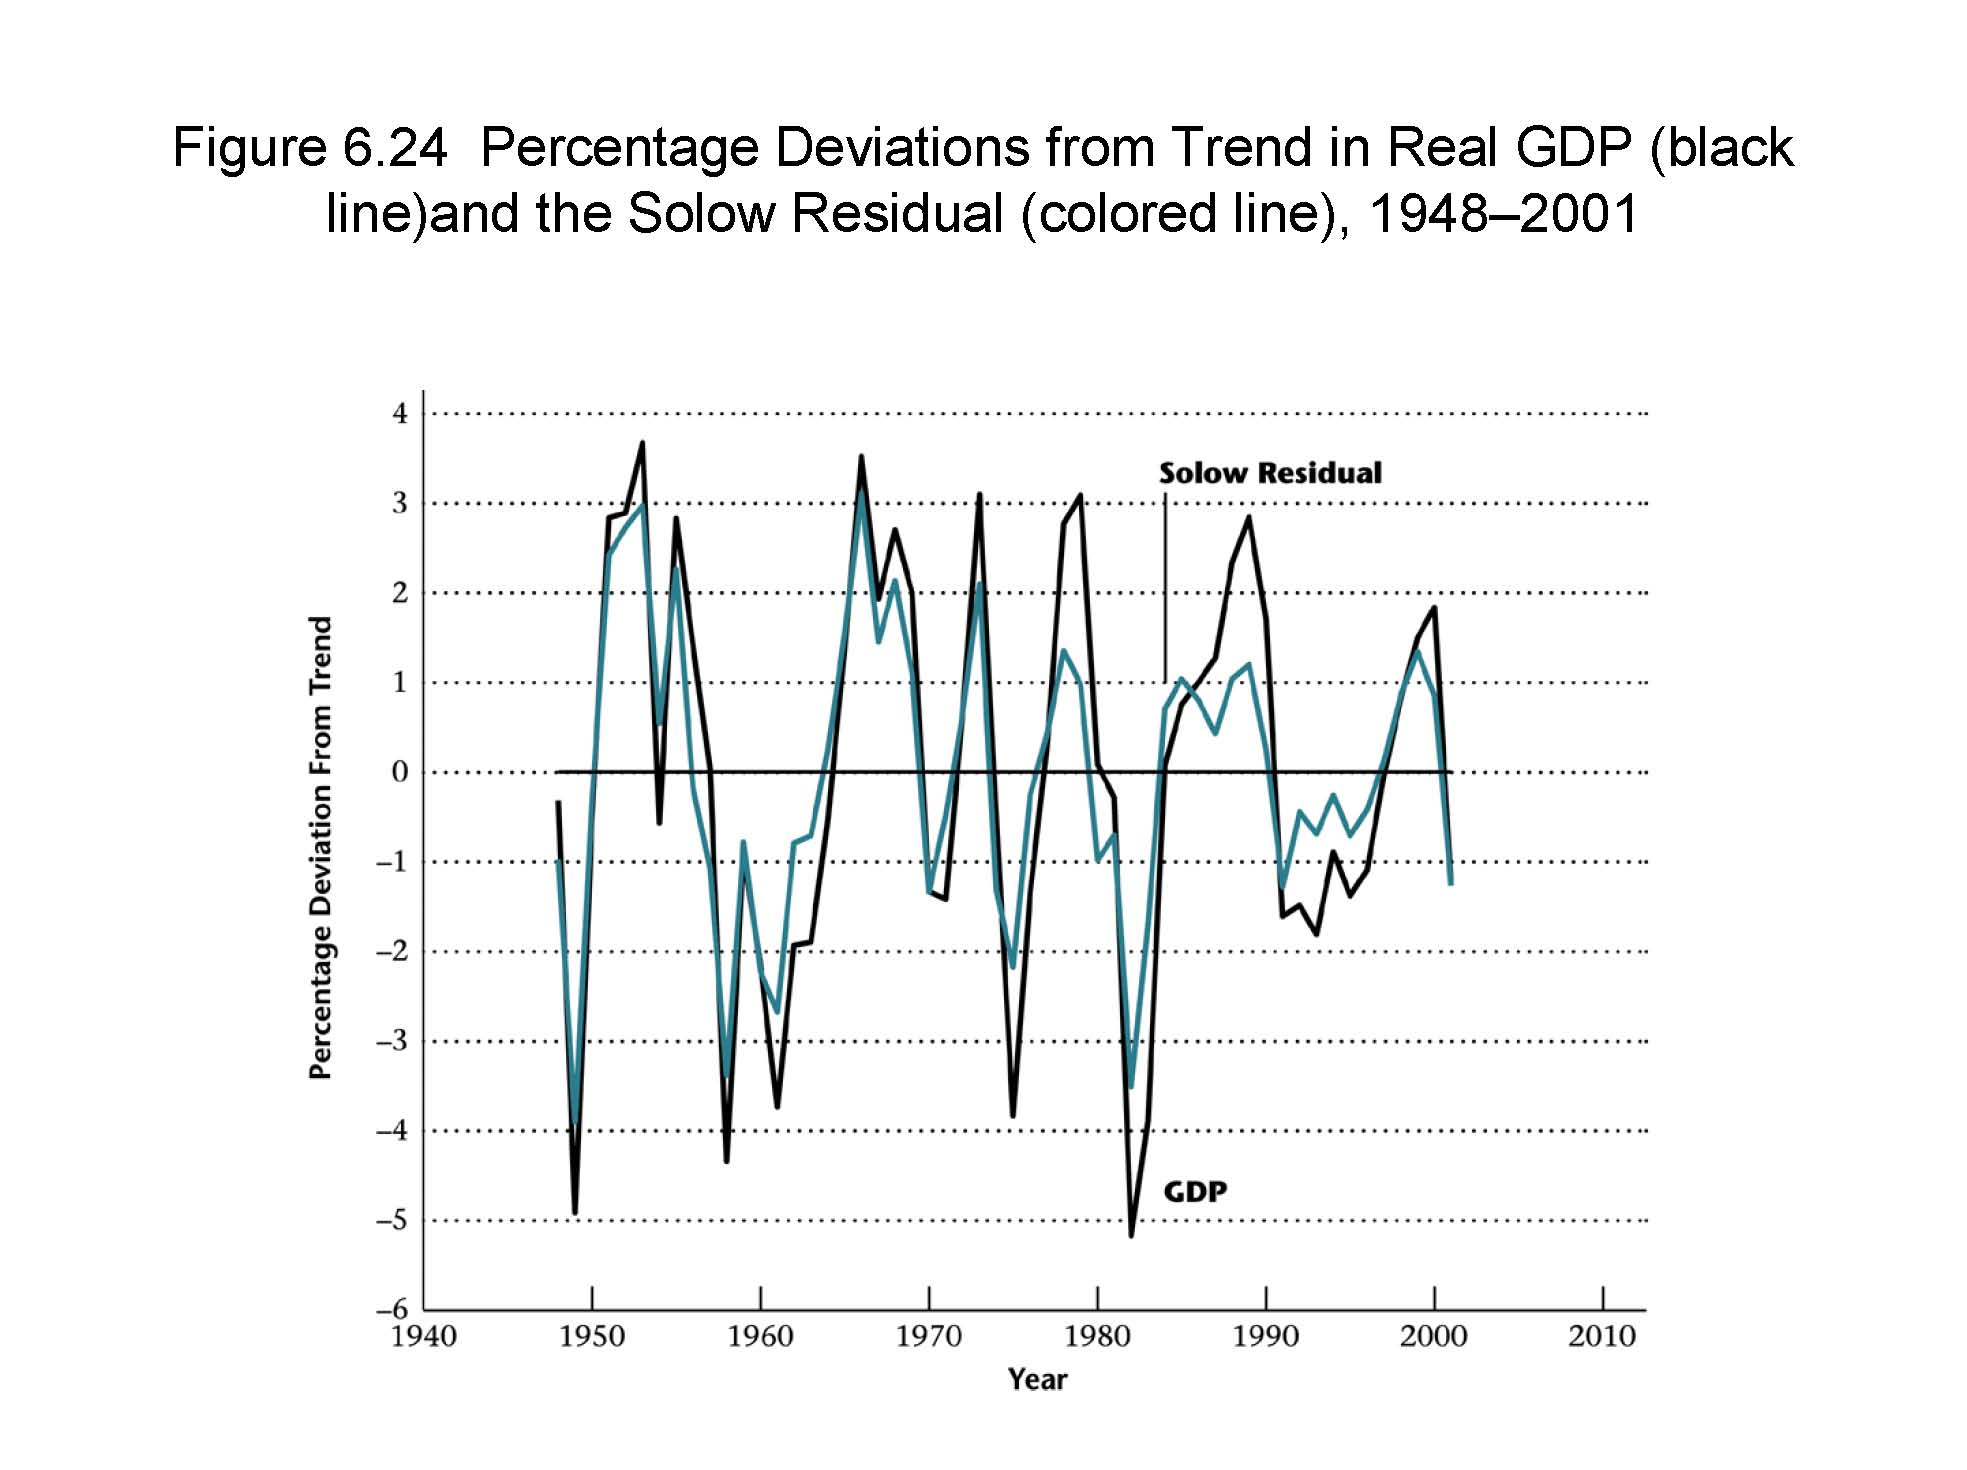
\includegraphics[width = 4.0in]{Fig6_11.jpg}
\end{figure}
\end{frame}



\begin{frame}

\frametitle{Introduction: Economic Growth and Business Cycles}

{\small{

$\Box$ Modern business cycle theory (Cooley and Prescott, 1995)
% Ref: Cooley Ch1: 29-33
\begin{itemize}
\item For a long time, study of short-term business cycles and study
of long-term growth were divorced;
\item Modern business cycle theory starts with the view that growth
and fluctuations are not distinct phenomena to be studied with
separate data and different analytical tools. This is due to the
developments:
\begin{enumerate}{\scriptsize{
\item Brock and Mirman's (1970) characterization of optimal growth
in an economy with stochastic productivity shocks;
\item The introduction of the labour-leisure choice into the basic
neoclassical model.}}
\end{enumerate}
\item The artificial economies are constructed to mimic important
aspects of the behavior through time of actual economies. Therefore,
they are useful laboratories for studying the business cycle and for
studying economic theory;
\item In the rest of this session, we study Hansen's benchmark
real business cycle model, in which the most common element is the
neoclassical model of economic growth --- the marriage of economic
theory and empirical observation.
\end{itemize}
}}
\end{frame}


\section{Hansen's Benchmark Real Business Cycle Model}

\subsection{The Environment}

\begin{frame}

\frametitle{Hansen's Benchmark Real Business Cycle Model (The
Environment)} \vskip 0.1in

\textcolor{blue}{Preferences:}

The model economy is populated by infinitely-lived households. The
preferences of households are assumed to be identical. Households
maximize the expected utility over life time:

\begin{equation}\label{Eq3.1}
U(C_t,N_t)=E_{t}\sum_{t=0}^\infty\beta^t\biggl(\frac{C_t^{1-\eta_{c}}-1}{1-\eta_{c}}-AN_t\biggr),\qquad
0<\beta<1\qquad \eta_{c}>0
\end{equation}

where $C_t$ and $N_t$ are consumption and labour respectively,
$\beta$ is the discount factor that households apply to future
consumption, and $\eta_{c}$ is the coefficient of relative risk
aversion.\\\vskip 0.1in


\end{frame}

\begin{frame}

\frametitle{Hansen's Benchmark Real Business Cycle Model (The
Environment)} \vskip 0.1in

\textcolor{blue}{Technology:}

The technology is defined as a standard Cobb-Douglas production
function:

\begin{equation}\label{Eq3.2}
Y_t=Z_tK_{t-1}^{\alpha}N_t^{1-\alpha}
\end{equation}

where $Z_t$ is total factor productivity (TFP) which is exogenously
evolving according to the law of motion:

\begin{equation}\label{Eq3.3}
logZ_t=(1-\psi)logZ^{ss} + \psi logZ_{t-1}+\epsilon_t, \qquad
\epsilon_t\sim i.i.d.(0,\sigma^2)
\end{equation}

\noindent where $\psi$ and $Z^{ss}$ are parameters, and
$0<\psi<1$.\smallskip
\end{frame}

\begin{frame}

\frametitle{Hansen's Benchmark Real Business Cycle Model (The
Environment)} \vskip 0.1in

\textcolor{blue}{Technology:}

As in a neoclassical growth model, capital stock depreciates at the
rate $\delta$, and households invest a fraction of income in capital
stock in each period. This amount of investment forms part of
productive capital in current period. Therefore the law of motion
for aggregate capital stock is

\begin{equation}\label{Eq3.4}
K_t=(1-\delta)K_{t-1} + X_t,\qquad 0<\delta<1
\end{equation}

\pause

\textcolor{blue}{Aggregate resource constraint:}

\begin{equation}\label{Eq3.5}
Y_t =C_t+X_t
\end{equation}

\end{frame}

\subsection{The FOCs}

\begin{frame}

\frametitle{Hansen's Benchmark Real Business Cycle Model (The FOCs)}
\vskip 0.1in

\textcolor{blue}{The Bellman equation:}\\
The model can be written as a Bellman equation of the form

\begin{equation}\label{Eq3.6}
V(K_{t-1},Z_{t}) = \max_{C_t, X_t, K_t, N_t}
[\frac{C_t^{1-\eta_{c}}-1}{1-\eta_{c}}-AN_{t} + \beta
E_{t}V(K_{t},Z_{t+1})]
\end{equation}

s.t.

\begin{eqnarray*}
Y_t &=& C_t+X_t\\
Y_t &=& Z_tK_{t-1}^{\alpha}N_t^{1-\alpha}\\
K_t &=& (1-\delta)K_{t-1} + X_t\\
logZ_t &=& (1-\psi)logZ^{ss} + \psi logZ_{t-1}+\epsilon_t
\end{eqnarray*}

\end{frame}


\begin{frame}

\frametitle{Hansen's Benchmark Real Business Cycle Model (The FOCs)}
\vskip 0.1in


The FOC w.r.t. $K_{t}$
\begin{equation}\label{Eq3.7}
1 = \beta E_t[\bigl(\frac{C_t}{C_{t+1}}\bigr)^{\eta_{c}}R_{t+1}]
\end{equation}

The FOC w.r.t. to $N_{t}$
\begin{equation}\label{Eq3.8}
A =  C_t^{-\eta_{c}}(1-\alpha)\frac{Y_t}{N_t}
\end{equation}

and
\begin{equation}\label{Eq3.9}
R_t = \alpha\frac{Y_t}{K_{t-1}}+(1-\delta)
\end{equation}

where, $R_t$ is the gross real return of capital, which is equal to
the real return $r_t$ plus $(1-\delta)$, i.e. $R_t = 1+ r_t
-\delta$\footnote{Take note, later on we use $\hat{r_{t}}$
represents the deviation of $R_{t}$ from its steady state }.

\end{frame}

\subsection{The Complete Model Economy}

\begin{frame}

\frametitle{Hansen's Benchmark Real Business Cycle Model (The
Complete Model Economy)}

\begin{eqnarray*}
Y_t &=& C_t+X_t \\
Y_t &=& Z_tK_{t-1}^{\alpha}N_t^{1-\alpha} \\
K_t &=& (1-\delta)K_{t-1} + X_t\\
1 &=& \beta E_t[\bigl(\frac{C_t}{C_{t+1}}\bigr)^{\eta_{c}}R_{t+1}] \\
\label{Eqe}
A &= & C_t^{-\eta_{c}}(1-\alpha)\frac{Y_t}{N_t}\\
R_t &=& \alpha\frac{Y_t}{K_{t-1}}+(1-\delta)\\
logZ_t &=& (1-\psi)logZ^{ss} + \psi logZ_{t-1}+\epsilon_t, \qquad
\epsilon_t\sim i.i.d.(0,\sigma^2)
\end{eqnarray*}


\end{frame}

\subsection{The Steady State}

\begin{frame}

\frametitle{Hansen's Benchmark Real Business Cycle Model (The Steady
State)}


\begin{eqnarray}
Y^{ss} &=& C^{ss}+X^{ss}\\
Y^{ss} &=& Z^{ss}(K^{ss})^{\alpha} (N^{ss})^{1-\alpha} \label{Eq3.11}\\
X^{ss} &=& \delta K^{ss} \\
R^{ss} &=& \frac{1}{\beta}\\
A &=&
\frac{1}{(C^{ss})^{\eta_{c}}}(1-\alpha)\frac{Y^{ss}}{N^{ss}}\label{Eq3.14}\\
K^{ss} &=& \biggl(\frac{\alpha
Z^{ss}}{R^{ss}-1+\delta}\biggl)^{\frac{1}{1-\alpha}}N^{ss}
\end{eqnarray}

\end{frame}

\subsection{The linearized Model}

\begin{frame}

\frametitle{Hansen's Benchmark Real Business Cycle Model (The
log-linearized Model\footnote{A small letter with \emph{hat}
represents the deviation from its steady state.})}
\begin{eqnarray}
\hat{y_t} &=& \frac{C^{ss}}{Y^{ss}}\hat{c_t} + \frac{X^{ss}}{Y^{ss}} \hat{x_t}\\
\hat{y_t} &=& \hat{z_t}+\alpha \hat{k}_{t-1}+(1-\alpha)\hat{n_t}\\
\hat{k}_t &=& \frac{X^{ss}}{K^{ss}} \hat{x}_t+(1-\delta)\hat{k}_{t-1} \\
0 &=& E_t [\eta_{c}(\hat{c}_t-\hat{c}_{t+1})+\hat{r}_{t+1}] \\
0 &=& -\eta_{c} \hat{c}_t+\hat{y}_t-\hat{n}_t \\
R^{ss}\hat{r}_t &=& \alpha
\frac{Y^{ss}}{K^{ss}}(\hat{y}_t-\hat{k}_{t-1}) \\
\hat{z}_t &=& \psi \hat{z}_{t-1}+\epsilon_t, \qquad \epsilon_t\sim
i.i.d.(0,\sigma^2)
\end{eqnarray}


\end{frame}

\section{Calibrating a Specific Model Economy}

\begin{frame}

\frametitle{Calibrating a Specific Model Economy}\vskip 0.1in

This section follows the three-step process (Cooley and Prescott,
1995) from the general framework described in the previous section
to quantitative measurements of the variables of interest ---
output, employment, investment, and so on.

\begin{itemize}
\item The first step is to restrict the model to display balanced
growth. That is, in steady state, capital, consumption and investment
all grow at a constant rate.\\
\item The second step is to define the
consistent measurements of the conceptual framework of the model
economy and the real data.\\
\item The parameter values of the model economy are then assigned
according to the measured data during the sample period of 1970 to
2000 (RSA).
\end{itemize}
\end{frame}


\begin{frame}

\frametitle{Calibrating a Specific Model Economy}\vskip 0.1in

\begin{itemize}
\item The annual aggregate capital depreciation rate $\delta$ is
obtained from annual averaged values of $\frac{X}{Y}$ and
$\frac{K}{Y}$. This yields an annual depreciation rate of 0.076, or
a quarterly rate of 0.019.\\
\item The standard real business cycle literature suggest that capital
and labour shares of output have been approximately constant. The
capital output share ($\alpha$) is equal to 0.26 obtained from the
steady state equation \eqref{Eq3.11}, whereas the labour output share
($1-\alpha$) is 0.74.\\
\item The discount factor $\beta$ is set equal to 0.99, as in Hansen
(1985), which implies an annual real interest rate of four percent
in steady state.\\
\item The coefficient of relative risk aversion $\eta_{c}$, is set
equal to one. The parameter $A$, in the utility function
\eqref{Eq3.1}, is equal to 2.6712, obtained from \eqref{Eq3.14}.
\end{itemize}
\end{frame}

\begin{frame}

\frametitle{Calibrating a Specific Model Economy}\vskip 0.1in

{\small{

The measurement of technology shock, also Known as Solow residual in
growth accounting literature (Solow, 1957), is computed from Eq.(\ref{Eq3.2}) as follows:
\begin{eqnarray}\label{Eq3.23} \nonumber
logZ_t-logZ_{t-1}&=&(logY_t-logY_{t-1}) - [\alpha(ln{K_t} - ln{K_{t-1}})  \\ 
&+& (1-\alpha)(logN_t-logN_{t-1})].
\end{eqnarray}
The parameter $Z^{ss}$, in the law of motion for TFP \eqref{Eq3.3},
is set equal to one. Therefore \eqref{Eq3.3} becomes a first-order
linear Markov process:\footnote{\scriptsize{We can assume that quarterly variations in capital stock are approx. zero. We therefore use real GNP and quarterly hours series (see Cooley \& Prescott, p.22.)}}

\begin{equation} \label{Eq3.24}
logZ_t=\psi logZ_{t-1} + \epsilon_t,\qquad \epsilon_t\sim
i.i.d.(0,\sigma^2)
\end{equation}

The persistence parameter $\psi$ is set equal to 0.95, which is
consistent with the literature (Hansen, 1985). From \eqref{Eq3.24}
one can compute a set of innovations of technology $\epsilon_t$.
These innovations have a standard deviation of 0.0083. }}
\end{frame}

\begin{frame}

\frametitle{Calibrating a Specific Model Economy}\vskip 0.1in

As shown in the table below, all parameters of the model have now
been assigned.


\begin{center}
\textbf{Parameters calibrated to the model economy}\\\medskip
\begin{tabular}{|c|c|c|c|c|c|c|c|}\hline
\multicolumn{ 5}{|c|}{\textit{technology}} &  \multicolumn{ 3}{c|}{\textit{preferences}} \\
\hline
$\alpha$ & $\psi$ & $Z^{ss}$ & $\delta$ & $\sigma_\epsilon$ & $\beta$ & $\eta_{c}$ & $A$\\
\hline 0.26 & 0.95 & 1.00 & 0.019 & 0.0083 & 0.99 & 1.00 &
2.6712 \\\hline
\end{tabular}
\end{center}


\end{frame}

\section{The Dynamics of the Model}

\begin{frame}

\frametitle{The Dynamics of the Model}\vskip 0.1in
\centering
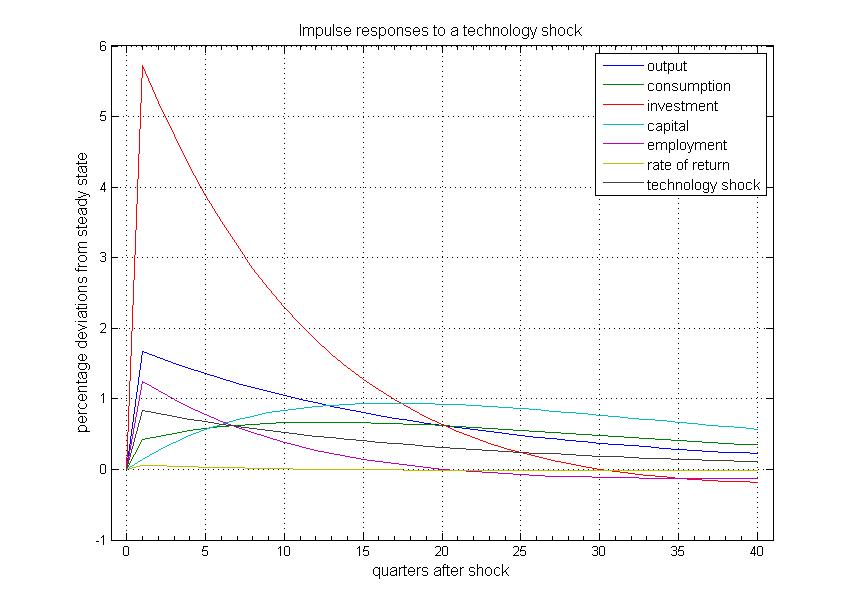
\includegraphics[width = 4.0in]{hansenrbctechshockcombinedslides.jpg}
\end{frame}
%%%\includegraphics[width = 4.0in]{Impulse_model.jpg}

\begin{frame}

\begin{table}
\caption{Cyclical properties}
\centering
\noindent\makebox{ {\scriptsize{
\begin{tabular}{lllllll}
\hline \hline
           &            & \multicolumn{ 2}{c}{standard deviation} &      &  \multicolumn{ 2}{c}{correlation} \\

           &            & \multicolumn{ 2}{c}{relative to output} &      &  \multicolumn{ 2}{c}{with output} \\

  Variable &            &       data &     rbc &             &       data &      rbc  \\
\hline
           &            &            &            &            &           &     \\

Output $(Y_t)$ &            &          1.00 &          1.00 &             &          1.00 &          1.00  \\

Consumption $(C_t)$ &            &       0.74 &       0.70 &             &       0.83 &       0.88  \\

Investment $(X_t)$ &            &       3.10 &       2.51 &            &       0.90 &       0.90  \\

Hours $(N_t)$ &            &       0.37 &       0.51 &             &       0.62 &      0.75  \\

Productivity $(Z_t)$ &            &   -   &       0.50 &             &      - &     1.00  \\

           &            &            &            &            &            &                 \\
\hline
%\multicolumn{9}{l}{Note: model 1 is simulated with a productivity shock. For model 2 a target leverage ratio}\\
%\multicolumn{9}{l}{shock and an equity premium shock are included in order to capture financial market}\\
%\multicolumn{9}{l}{properties in the data not explained by the traditional RBC theory. All variables, except} \\
\multicolumn{7}{l}{{\tiny{Note: all variables, except for rates, are in log real terms and are detrended using}}}\\
\multicolumn{7}{l}{{\tiny{the HP filter. Source: Cooley \& Prescott, 1995: cherry-picked from Table 1.1 and 1.2.}}}\\
%\multicolumn{7}{l}{{\tiny{}}}\\
\end{tabular}
} }}\end{table}

\end{frame}

%\begin{frame}
%\begin{center}
%\Huge{THE END}
%\end{center}
%\end{frame}

\end{document}
